\documentclass[compress,11pt]{beamer}
%\includeonly{pendel}
\usetheme{Ilmenau}
%\usetheme{fau-4-3}
%\usecolortheme{beaver}
%\beamertemplatenavigationsymbolsempty
\usepackage[ngerman]{babel}
\usepackage{marvosym}
\usepackage{multimedia}
\usepackage[utf8]{inputenc}
\usepackage{amsmath}
\usepackage{amsfonts}
\usepackage{amssymb}
\usepackage{graphicx}
\usepackage{esvect}
%\author{}
\title{EP Gruppe 8}
%\setbeamercovered{transparent}
%\setbeamertemplate{navigation symbols}{}
%\logo{}
%\institute{}
%\date{}
%\subject{}
\usepackage{verbatim}
\begin{document}
\section{A3: A-D-Wandler}
\begin{frame}
Schaltplan:




\end{frame}
\begin{frame}
Pin-Belegung des A/D-Wandlers:\\



\begin{itemize}

\item Betätigen des Schalters gibt Signal an den Clock-Pin und startet einmalig die Übersetzung
\item Über Pin 5 wird der Beginn der Übersetzung signalisiert
\end{itemize}
\end{frame}
\begin{frame}
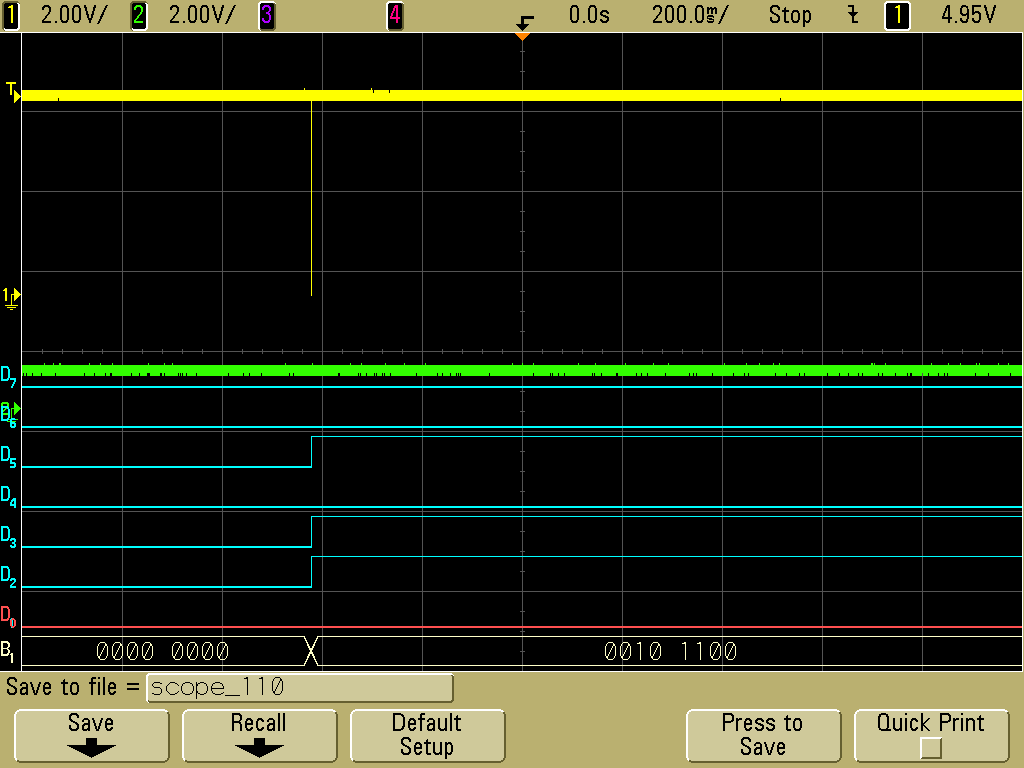
\includegraphics[width=.7\textwidth]{../vales_zeug/scope_110}\\
Beispiel: Wandlung von $U_{in} = 1 V$ Gleichspannung
\end{frame}
\begin{frame}
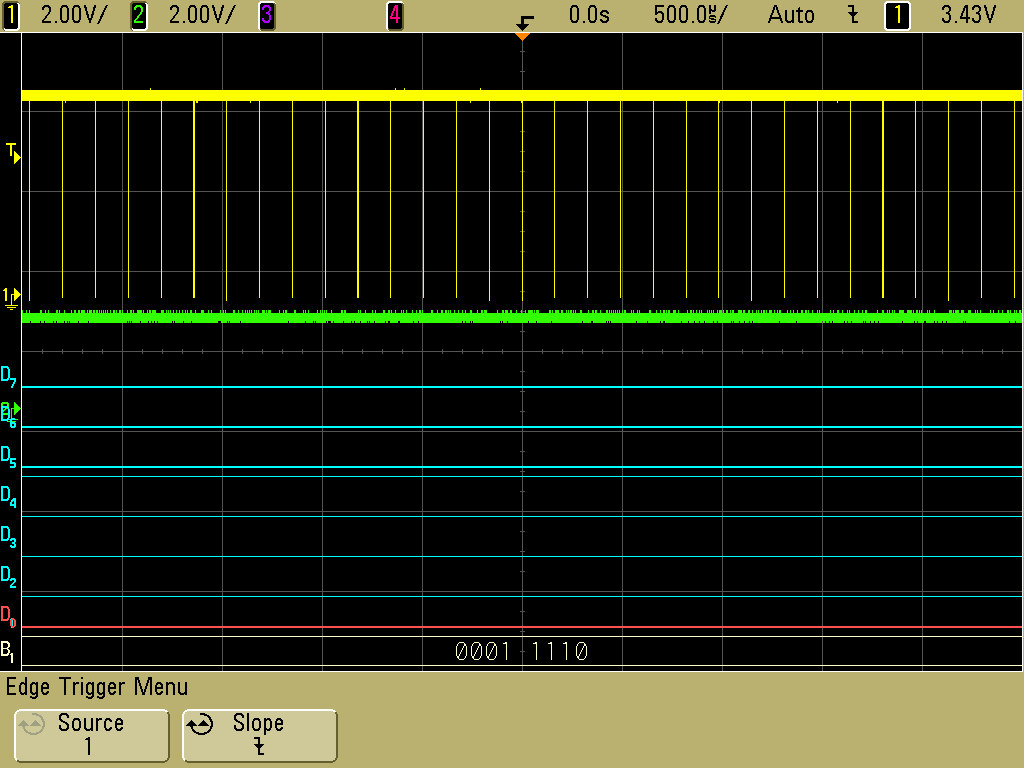
\includegraphics[width=.7\textwidth]{../vales_zeug/scope_114}\\
Durch das Umsetzen des Widerstandes von Pin 3 und Pin 20 zu Pin 3 und 5 kann eine regelmäßige Übersetzungsanweisung erzeugt werden $\Rightarrow$  Eingangssignal wird regelmäßig neu übersetzt
\end{frame}
\begin{frame}
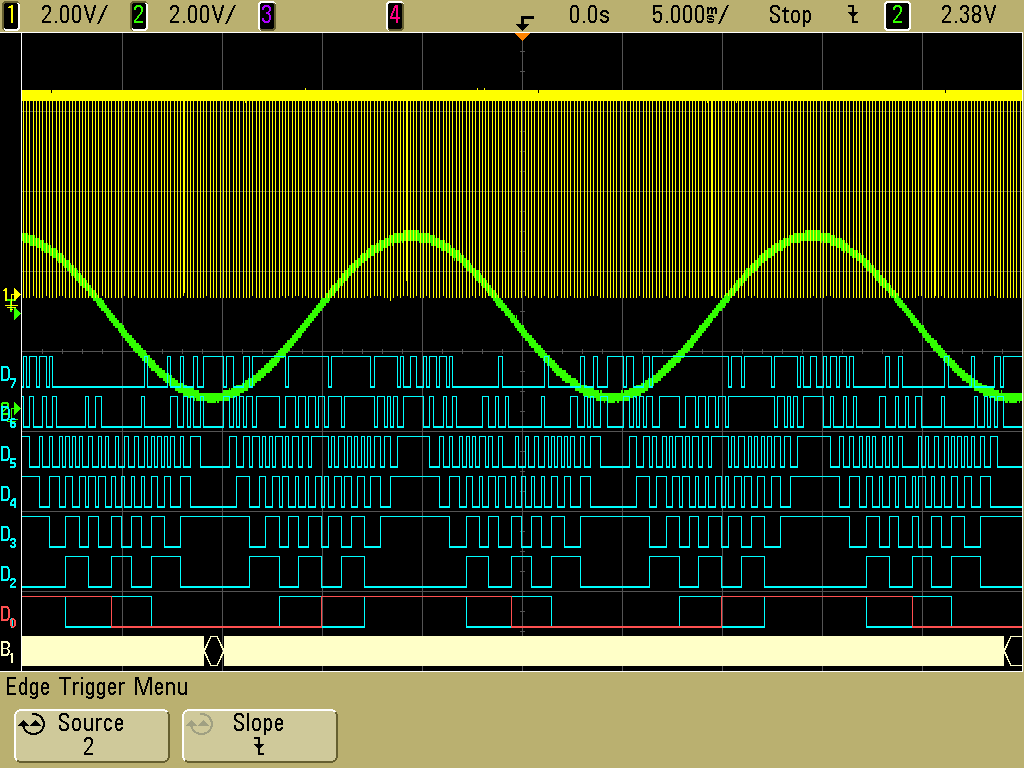
\includegraphics[width=.7\textwidth]{../vales_zeug/scope_115}\\
Wandlung einer Sinus-Spannung
\end{frame}
\begin{frame}
Exemplarisch gemessene Werte für die A/D-Wandlung:
\begin{tabular}{|c|c|}
\hline
$U_{in} in V$ & $N_{out}$  \\
\hline
1	&	44 \\
1.4 &	18 \\
2.3	&   30 \\
3.147	&	69 \\
\hline
\end{tabular}\\
Mit $N_{out} = \frac{U_{in}}{U_{LSB}}$ (Vorlesung) ergibt sich im Mittel: 
\begin{equation}
U_{LSB} = 0.055695 V
\end{equation}
\begin{block}{Randbemerkung}
Der erste Wert in der Tabelle ist möglicherweise fehlerhaft, die anderen drei Werte lassen fast auf einen parabelförmigen zusammenhang schließen (siehe nächste Folie)
\end{block}
\end{frame}
\begin{frame}
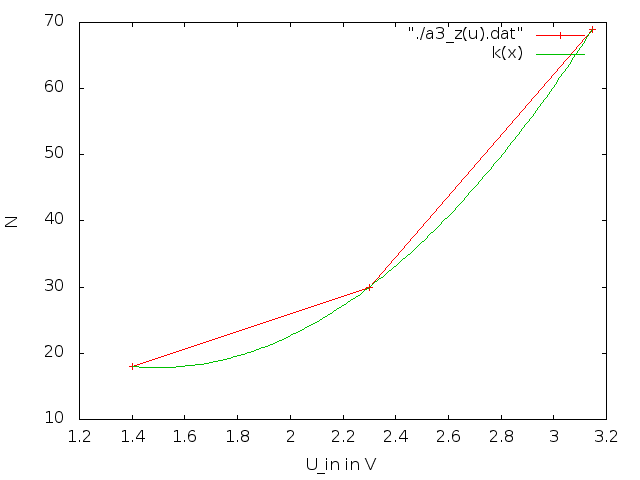
\includegraphics[width=.5\textwidth]{../plots/blub}
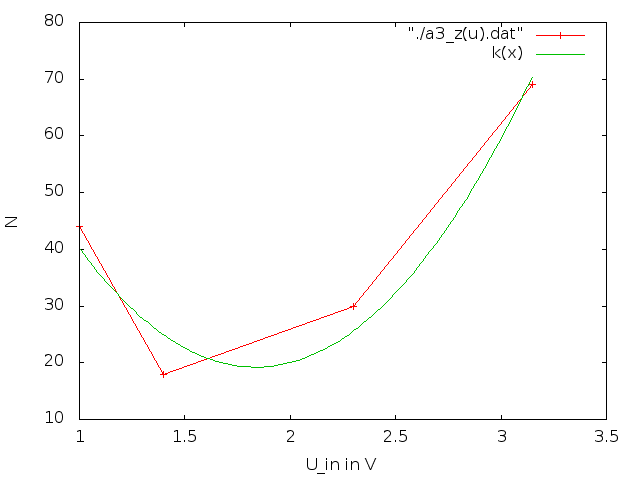
\includegraphics[width=.5\textwidth]{../plots/blub2}\\
\end{frame}
\end{document}